\chapter{Embedding Scheme in a browser} \label{scheme}

The Scheme development environment is the foundation for a number of fascinating applications in education and research. But executing Scheme program directly into the browser is not possible yet, since Scheme is not readily available in the browser. In such cases, JavaScript being de-facto of browser based applications, a JavaScript based and browser native implementation Scheme is desirable.

For this project we created Scheme in browser using JavaScript. It provides supports for some of the core language features with additional feature of interacting with DOM to enable scheme to interact with the browser.  The core of our environment is inspired by the scripting API \cite{javascripting} by taking the same approach to interact with other languages. 

\begin{figure}[ht]
	\begin{center}
		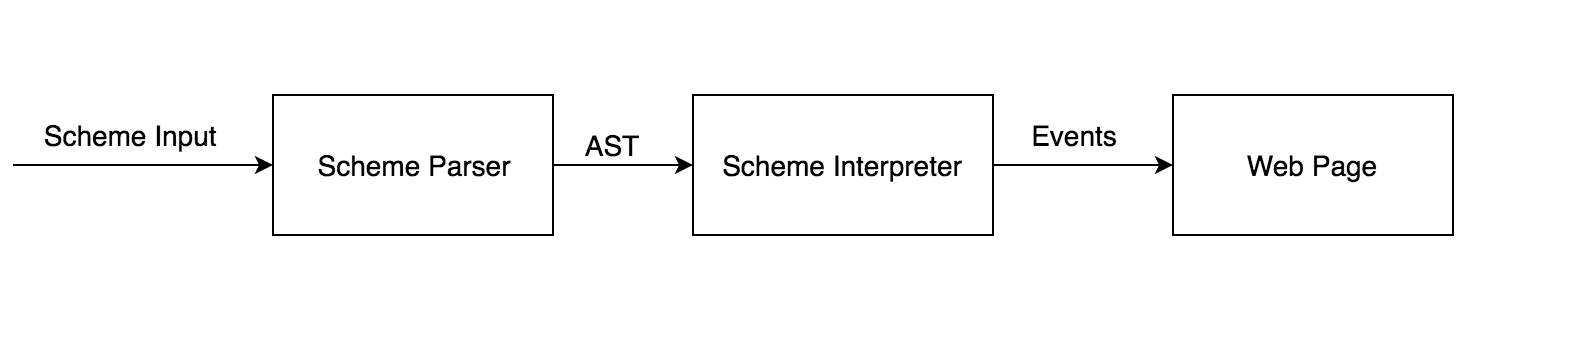
\includegraphics[width=\linewidth]{./images/SchemeEnvironmentusingJavaScript.png}
	\end{center}
	\caption{Scheme Environment using JavaScript: Architecture}
	\label{fig:SchemeEnvironmentusingJavaScript}
\end{figure}


As shown in Figure \ref{fig:SchemeEnvironmentusingJavaScript}, Our Scheme library takes web page's embedded Scheme scripts as input. Our plugin will parse and then interpret the input scripts using JavaScript. This interpreted Scheme code then interacts with the browser, to help render web pages with more dynamic behaviour. 

\section{Interpreter} 
As discussed in previous chapters, browsers do not have a readily available support for the Scheme. To help enable the browser to understand code written in the Scheme, we built a Scheme interpreter written in the JavaScript. Using our Scheme interpreter, browser will understand program written in the Scheme.

The Scheme code will be embedded into the web page using script tag as shown in the code Example \ref{fig:schemescript}, 

\begin{figure}[h]
	\begin{lstlisting} 
	<script type="text/scheme">
	(
	 (define square
	  (lambda (n) 
	   (console-log (* n n)
	  ) 
	 )
	)
		
	(square 6)
	)
	</script>
	\end{lstlisting}
	\caption{Scheme script example}
	\label{fig:schemescript}
\end{figure}



As shown in the code snippet in Figure \ref{fig:schemescript}, Scheme code can be added inside the webpage using "$<$script type="text/scheme" $>$ $<$/script$>$" script tag. Our interpreter supports multiple number of Scheme script tags.

In order for the browser to understand the Scheme, code snippet written inside Scheme script tags is parsed and interpreted by our browser plugin. In case, the browser plugin is unavailable then we need to include library reference of interpreter on the page, as shown in the example below, 

\begin{lstlisting}
	<script src="simple-scheme-interpreter.js">
\end{lstlisting}

If the browser plugin is available, then this script file is added by the browser plugin, so we don't have to worry about adding it in the web page.

The interpreter consists of two parts:

\subsection{Parser}

After code snippets from script tags is read, first thing our library does is to parse the input code using PEG.JS and get the Abstract Syntax Tree (AST). The interpreter then uses this AST to interpret the code.

\subsubsection{PEG.js}

We used a PEG.js library to create a parser for the Scheme \cite{pegjs}. PEG.js is simply a parser written in the JavaScript. We can use it to create parsers for complex data and computer languages. A sample PEG.js grammar used to parse the Scheme code is shown in the code example \ref{fig:schemepeg},


\begin{figure}[h]
	\begin{lstlisting}  

	var parser = PEG.buildParser( 
	' start = multiexpression;\
	validchar = [a-zA-Z_?!+\\-=@#$%^&*/.];\
	spaces = \`` \''*;\
	newline = [\\n]*;\
	digit = [0-9];\
	atom =    spaces newline chars:validchar+ spaces 
	    newline   { return chars.join(\``\''); }\
	    / spaces newline numbers:digit+ spaces newline     
        { return parseInt(numbers.join(\``\'')); };\
    
	list = spaces newline \``(\'' spaces newline 
	   expressionss:multiexpression+ newline spaces\``)\''
	   spaces newline { return expressionss; };\
	   expressions = spaces newline 
	   lists:list+ newline spaces { return lists };\
	   multiexpression = atom / expressions ;');
	\end{lstlisting}
	\caption{Scheme PEG.js parser}
	\label{fig:schemepeg}
\end{figure}

Using the grammar shown in Figure \ref{fig:schemepeg}, Scheme code is parsed into AST using a following statement.

\begin{lstlisting}
	var PegAST= parser.parse(s);
\end{lstlisting}




\subsection{Interpreter}

AST generated by the parser is interpreted by our interpreter written in the JavaScript, as shown in the code example below,


\begin{lstlisting}
	var pegRet = schemeInterpreter.interpret(PegAST);
\end{lstlisting}


The interpreted output is either DOM event or JavaScript code which the browser understands.

\section{Scheme for Browser} 

Following the R5RS standard \cite{Adams:1998:RRA:290229.290234}, variables are  blocked scoped in the program. 

Blocks can be created with let, or define expressions, like:


\begin{lstlisting}
	(let ((x 10)
		(y 20))
	
	(foo x y))
\end{lstlisting}


In the example shown above, variable x and y are blocked scoped. Both x and y are available to function foo.

Like the universal Scheme, our implementation of the Scheme supports following features:
\begin{itemize}
	\item {\textbf{Basic Types}}
	\begin{itemize}
		\item Integer
		\item Real
		\item Number
		\item String
		\item List
		\item Char
	\end{itemize}
\end{itemize}

\begin{itemize}
	\item{\textbf{Control structure}}
	\begin{itemize}
		\item Conditional
		\begin{itemize}
			\item if then else cond case
		\end{itemize}
		\item Loop
		\begin{itemize}
			\item do let(named let) dotimes
		\end{itemize}
		\item Assignment
		\item eval
	\end{itemize}
\end{itemize}

It also provides special language syntax to interact with the browser's DOM. We chose to include basic, most used browser functions for our Scheme DOM API. This is only available for browser. 

\begin{itemize}[label={}]
	\item First.
	\item Second.
\end{itemize}

\begin{itemize}
	\item {\textbf{Browser  Functions}}
	\begin{itemize}
		\item {Dialog}
			\begin{itemize}
				\item {(alert msg)}
				   \begin{itemize}[label={}]
				   	\item  Similar to, ``window.alert" function.
				   \end{itemize}
			\end{itemize}
		
			\begin{itemize}
				\item {(confirm msg)}
				\begin{itemize}[label={}]
					\item  Similar to, ``window.confirm" function. It returns a boolean value.
				\end{itemize}
			\end{itemize}
	\end{itemize}

	\begin{itemize}
		\item {Event}
		\begin{itemize}
			\item {(add-handler! selector event proc)}
            \begin{itemize}[label={}]
            	\item  Attaches an event handler to the specified selector. It returns the handler function, which handles the event.
            \end{itemize}
		\end{itemize}
		
		\begin{itemize}
			\item {(remove-handler! selector event js-handler)}
			\begin{itemize}[label={}]
				\item  Removes the attached event handler from the specified selector.
			\end{itemize}
			\begin{itemize}
				\item {eg (define h (add-handler! "$#$button1" "click" (lambda (ev) ...)))}
				\item {eg (remove-handler! "$#$button1" "click" h)}
			\end{itemize}
		\end{itemize}
	\end{itemize}

	\begin{itemize}
		\item {Element}
		\begin{itemize}
			\item {(element-visible? elem)}
				\begin{itemize}[label={}]
					\item  Returns the visibility of the specified element.
				\end{itemize}
			\item {(element-toggle! elem)}
			    \begin{itemize}[label={}]
			    	\item  Toggles the visibility of the specified element.
			    \end{itemize}
			\item {(element-hide! elem)}
			    \begin{itemize}[label={}]
			    	\item  Hides the specified element.
			    \end{itemize}
			\item {(element-show! elem)}
			    \begin{itemize}[label={}]
			    	\item  Shows the specified element.
			    \end{itemize}
			\item {(element-remove! elem)}
			    \begin{itemize}[label={}]
			    	\item  Removes the specified element.
			    \end{itemize}
			\item {(element-update! elem html)}
			    \begin{itemize}[label={}]
			    	\item  Updates the specified element with the provided html.
			    \end{itemize}
			\item {(element-replace! elem x)}
			    \begin{itemize}[label={}]
			    	\item  Replaces the specified element with provided value x.
			    \end{itemize}
			\item {(element-insert! elem x)}
			    \begin{itemize}[label={}]
			    	\item  Appends the specified element with provided value x.
			    \end{itemize}
			\item {(element-select elem)}
			    \begin{itemize}[label={}]
			    	\item  Returns the specified element.
			    \end{itemize}
		\end{itemize}
	\end{itemize}
\end{itemize}

Apart from providing DOM APIs for the browser, our Scheme interpreter supports interface to some of the basic JavaScript functions as shown:


\begin{itemize}
	\item{\textbf{JavaScript language interface}}
	\begin{itemize}
		\item {(js-eval str)
			\begin{itemize}[label={}]
				\item  Evaluate str as JavaScript code}
			\end{itemize}
			 
	\end{itemize}

	\begin{itemize}
		\item Console
		\begin{itemize}
			\item {(console-log obj1 ...)}
			    \begin{itemize}[label={}]
			    	\item  Similar to, JavaScript's ``console.log", it logs events to the console.
		        \end{itemize}
			\item {(console-debug obj1 ...)}
			    \begin{itemize}[label={}]
			    	\item  Alias for ``console-log''
			    \end{itemize}
			\item {(console-error obj1 ...)}
			    \begin{itemize}[label={}]
			    	\item  Logs the error message.
			    \end{itemize}
		\end{itemize}
\end{itemize}
\end{itemize}


\section{Approach}

Our Scheme interpreter uses the browser plugin approach to help the browser to understand the Scheme code on the web page.

\subsection{Browser Plugin } 
For this approach, the browser plugin (supported by Firefox, and Chrome) will push the instance of PEG.js parser and our Scheme interpreter into every newly opened browser tab. In this way, user doesn't have to worry about adding the library script on the page. Our library will then parse and interpret all the code enclosed within Scheme script.


\begin{figure}[h]
	\begin{lstlisting}  
	<script type=``text/scheme''>
	(alert ``Hello World'')
	(console-log ``Hello World'')
	</script>
	\end{lstlisting}
	\caption{Scheme browser plugin example}
	\label{fig:browserpluginscheme}
\end{figure}


As shown in Figure \ref{fig:browserpluginscheme}, we don't need to add any external libraries into our web page. Browser plugin will take care of interpreting the Scheme scripts. After executing the code in Figure \ref{fig:browserpluginscheme} in the browser with our plugin installed, will alert user with ``Hello World" as text.


\subsubsection{JS Library}

When the plugin is unavailable in the browser, the Scheme support is achieved in the web page by including Scheme interpreter and parser libraries in the web page itself. When the web page is loaded in the browser, libraries will read code snippet inside Scheme script and will interpret it, as shown in the Figure \ref{fig:browserwithoutpluginscheme}. 

\begin{figure}[h]
	\begin{lstlisting} 
	<script src=``./simple-scheme-interpreter.js''/> 
	<script type=``text/scheme''>
	(alert ``Hello World'')
	(console-log ``Hello World'')
	</script>
	\end{lstlisting}
	\caption{Scheme without browser plugin example}
	\label{fig:browserwithoutpluginscheme}
\end{figure}



As shown in code snippet in the Figure \ref{fig:browserwithoutpluginscheme}, instance of PEG.js and Scheme interpreter is embedded directly in the web page. Interpreter will interpret ``(alert "Hello World") and it will show an alert on the screen with ``Hello World" as text.